\chapter{Turbulent Heating}\label{app:4}


By including time dependence and shear viscosity, $\mu$, into the stellar wind momentum equation of section \ref{x} we get the Navier-Stokes equation
\begin{equation}
\rho \left(\frac{\partial v}{\partial t}+v. \nabla v\right)=-\nabla P + \mu \nabla ^2{v} + f_{other}
\end{equation} 
where $f_{other}$ represents other forces such as gravity, radiation pressure and the unknown wind driving force(s), and $\nabla ^2$ is the vector Laplace operator. In most astronomical settings we expect the viscous term to be unimportant. This can be seen by considering the ratio of the inertial term to the viscous term in the Navier-Stokes equation \cite{shu_1992}:
\begin{equation}
\frac{\rho v.\nabla v}{\mu \nabla ^2 v} \thicksim \frac{\rho U^2 /L}{\mu U / L^2}=\frac{UL}{\nu} \equiv Re,
\end{equation} 
where $U$ is a typical flow speed, L is the macroscopic length of the problem, $R_{e}$ is the Reynolds number, and $\nu \equiv \mu /\rho$ is called the kinematic viscosity. The shear viscosity is defined as
\begin{equation}
\mu \sim mv_{T}/\sigma
\end{equation} 
where $v_{T}$ is the thermal speed and $\sigma$ is the typical collision cross section. Therefore the kinematic viscosity has the unit of velocity times length where,
\begin{equation}
\nu \sim v_{T}l
\end{equation} 
and $l$ is the collision mean free path. The Reynolds number can then be written as \cite{1992pavi.book.....S}
\begin{equation}
Re \sim \frac{UL}{v_{T}l} \gg 1 \ \ \ \ \mathrm{when} \ \ \ \ \ U \sim v_{T}
\end{equation} 
In other words, in stellar winds where the flow speeds are sonic or supersonic, the Reynolds number must be large and viscous forces are much less important than inertial effects. These high [$Re \gg 10^3 \ \rm{to} \ 10^4$ i.e. the Reynolds number values associated with the onset of turbulence \cite{1998ISAA....4.....H}] Reynolds numbers then produce turbulent flow resulting in the formation of eddies and other flow instabilities.\\
\\
The rate at which energy is fed into the largest eddies per unit mass equals
\begin{equation}
\epsilon \sim \frac{U^2}{L/U} = \frac{U^3}{L}
\label{eq:1a}
\end{equation} 
This energy can neither accumulate nor dissipate viscously so the only other route for it is to be progressively transferred to eddies of smaller and smaller scales. If these smaller eddies have a scale $\lambda$ and velocity $v_{\lambda}$ then the energy that cascades from the large to the small per unit mass is
\begin{equation}
\epsilon \sim v_{\lambda}^3/\lambda
\label{eq:1b}
\end{equation}
Combining equation \ref{eq:1a} and \ref{eq:1b} gives Kolmogorov's law:
\begin{equation}
v_{\lambda} \sim U\left(\frac{\lambda}{L}\right)^{1/3}
\end{equation}
The process of transferring energy from large eddies down to smaller eddies continues until the scale of the turbulance is small enough for viscous action to become important and dissipation as heat to occur. 

\begin{figure}[!ht]
\centering 
         \includegraphics[trim=0pt 230pt 0pt 210pt,clip, width=12cm, height=9cm]{/home/eamon/thesis/thesis_template/appendix/turb.ps}
\caption[Kolmogorov spectrum]{Kolmogorov spectrum: The energy (turbulent energy) spectrum as a function of eddie size $\lambda$ that depends on the 1/3 power of $\lambda$.}
\label{fig:app4}
\end{figure}

